To build a Human-in-the-Loop grasp planning system, we need an underlying grasp planner that is responsive to human input and runs in near real time. Because we have a human in the loop, it is acceptable for the planner to generate grasps that are either not suitable for the object or that are not reflective of the users intent some of the time, as the user can reject them. However, because this platform is meant to be used through a low bandwidth, somewhat noisy input, it is important that there not be a large number of grasps for the user to reject. 

In this chapter, we describe the online grasp planner used in our system and the modifications which we have made to improve to its performance under the conditions of our system. This work was initially presented in \cite{Weisz2012}. In particular, it is difficult for the user to reject grasps which appear stable but which are likely to fail when there are errors in object localization that might interfere with realizing the grasp which is displayed to them. Here, we present a detailed description of the basis of our online grasp planning system, an analysis of the grasps that are produced by the online planner without considering the problems posed by object localization errors, and the method we use to ameliorate this difficulty. 

\section{Grasp Planning With Contact Points}

Analytical models analyzing the probability of grasp success have not been found, and so far the most generic methods involve sampling. The configuration space of the ``grasping'' problem has several formulations, but the two most common are potential contact points or hand configurations. In analyzing potential contact points, one can either analyze points on the hand or on the object. There are numerous considerations that one can take into account that make intuitive heuristic sense, including geometric concerns such as local flatness. 

Historically, it has been common to analyze the forces that can be applied at each contact point. There are no perfect models for this analysis. Models are generally classified by the physical systems that they roughly approximate. A point contact model assumes that the contact point can only apply forces in the direction opposite the normal of the surface on which it contacts. This is a conservative model. In order to generate a stable grasp from point contacts, it is necessary that any small (i.e., differential) motion cause the object to overlap the proposed contact points. This is called \emph{form closure}. When this is the case, it is also the case that the positive span of the set of wrenches produced by transforming the contact normals to some common references frame covers all of $\mathbb{R}^6$. This is an example of \emph{force closure}. For point contacts, these constraints are \emph{duals}, and one strictly implies the other. For the rest of the contact models, which take friction into account, this is not the case - one can have \emph{force close} without \emph{form closure}. 

This model is simple and conservative, but unfortunately it is too conservative to be useful for arbitrary objects. If rotations are considered, cylindrical objects cannot be grasped through \emph{form closure}, because there is no contact normal that can oppose rotations along the length of the cylinder. More generic models include frictional forces in addition to pure normal forces. Point-contact-with-friction models allow friction to be employed at each of the contact points in the plane orthogonal to the normal. In this case, the forces that can be produced at the contact point through friction are related to the normal force through the friction coefficient of the surface. This creates a cone of potential forces that can be created as the normal forces are scaled up. 

Further, if the contacting surface is assumed to be `soft' so that one surface conforms to another forming a contact patch, rather than a point, the contact can also apply torque around the normal direction.  If the surface is significantly softer, the patch can be modeled as a set of points on the perimeter of the patch. These points will be able to apply torques around all three dimensions with respect to the original contact point, and forces along any direction in the positive halfspace of the surface normal.  

In order to analyze how the contact forces affect the object, the forces and torques need to be summed up in the same reference frame. Most often, they are transformed to the centroid of the surface mesh or to the center of mass, if known. Transforming the cone of forces that can be produced by the point with friction model is difficult because it cannot be represented by a linear model, and so the linear transform to the new reference frame leads to a complex representation. In order to avoid this, the cone is represented by a simple linearization, making the base of the shape a regular polygon rather than a circle. Then the potential forces can be represented by the edges from the contact point to the points on the perimeter, normalized by the number of edges. This is illustrated in Fig. \ref{fig:friction-cone-linearization}. 

\begin{figure}
\centering
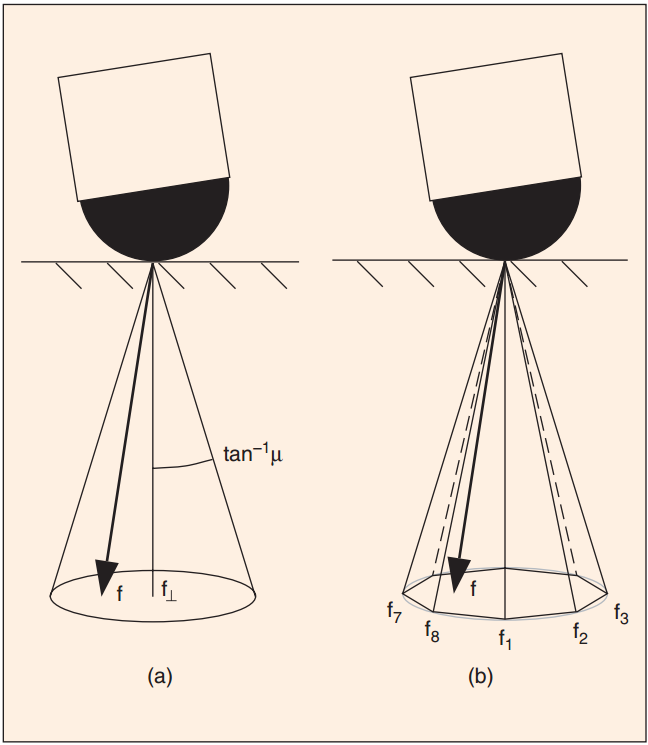
\includegraphics[width=6cm]{friction_cone_linearization.png}
\caption{The cone of forces that can be produced by a contact point can be represented by a simple linearization, making the base of the shape a regular polygon rather than a circle.  This illustration is taken from \protect\cite{Miller2004}}
\label{fig:friction-cone-linearization}
\end{figure}



\section{Grasp Wrench Spaces}
To characterize the contribution of the contact wrenches to constructing stable grasps, we need a way to analyze the entire set of wrenches holistically.  Irrespective of the contact model used, so long as it is linearized, the contacts can be summed up in the same reference frame, and all potential forces that could possibly be generated by these contact points can be represented. This set of forces is called the ``Grasp Wrench Space.''
In plain terms, the Grasp Wrench Space represents the set of wrenches that can be applied by this grasp.  A key criterion that is often used to define a successful grasp is the ability to generate a wrench in an arbitrary direction, which is the generic definition of \emph{force closure}.  This property is considered fundamental in grasp analysis because it provides a simple, necessary condition for grasp stability\cite{SalisburyThesis}. 
 
\section{The $\epsilon_{GWS}$ Quality Metric}
The $\epsilon_{GWS}$ metric of grasping extends force closure from a binary property which is or is not satisfied to a measure of how stable a grasp is with respect to grasp forces. The $\epsilon_{GWS}$ measure is one of the most widely cited 
benchmark metrics in the grasp planning field\cite{ferraricanny}.  Formally, for a set of contact wrenches $C\subset R^6$, one can define the neighborhood ball $B(\epsilon)$ and wrench space metric $\epsilon_{GWS}$ as follows: 
$$B(\epsilon) = \{x\in R^6 \mid \  ||x||_{L2} < \epsilon\}$$ 
$$\epsilon_{GWS} (C) = \max_{ \epsilon } [B(\epsilon )\subseteq  convexhull(C)] $$\par
Any grasp that does meet the minimum requirement of an $\epsilon_{GWS} > 0$ cannot apply force in some direction, which means that some infinitely small force in that direction will cause the object to begin to move. This quality metric is popular largely because it analytically addresses  an intuitively necessary condition for grasp stability, the ability to resist force perturbations.   One shortcoming of this measure is that it is sensitive to the choice of center of mass of the object.  A variant of this measure is to consider the volume of $convexhull(C)$, denoted $V_{GWS}$ in this work.  This variant functions as an approximation of the average case $\epsilon_{GWS}$ over many estimations of the center of mass of the object. \par

\section{Optimization Based Grasp Planning}
Given a quality measure that is computationally tractable, it is feasible to create a stochastic optimization based grasp planner. Sampling potential contact points directly on the object leaves the problem of finding a hand configuration that matches that contact configuration unsolved. For the generic case of arbitrary hands, this problem is difficult and unsolved. Similarly, sampling candidate contact points on the hand is equally intractable, because most hand configurations produce no contacts at all. To make the problem tractable, the state space needs to be relatively low dimensional and the quality metric must generate valid, informative values on most of that state space. 

\subsection{Potential Contact Quality Function}
This lab produced such an optimization based planner using simulated annealing to optimize cost functions that derive from the $\epsilon_{GWS}$ in \cite{Ciocarlie2008}. To make the quality metric accessible to this method and more computationally tractable, the potential contact points on the hand are projected to the object and the resulting contact wrenches are weighted by their distance and the agreement of their normal directions. This ``potential contact'' quality function creates a smoother optimization function. 

\subsection{Implications For Pose Error Robustness}
\label{sec:implications_for_robustness}
\begin{figure}[h]
\begin{center}
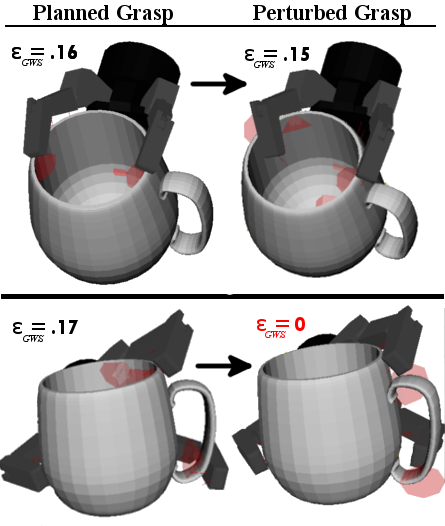
\includegraphics[height=80mm,width=80mm]{mug_grasps_combined_4.png}
\caption{An example of a grasp where the $\epsilon_{GWS}$ is consistent with respect to the common localization errors, and one where it is not.}
\label{fig:pose_robust_mug}
\end{center}
\end{figure}

A stochastic optimization based approach is capable of escaping local minima in complex, nonconvex optimization functions like the projected distance and alignment between nonconvex shapes. However, the net affect of the optimization procedure is still to approximately follow a gradient. We should thus expect that the most optimal grasps that are found should usually be found in areas where the quality function is fairly smooth and the basin of attraction is wide. Given the quality function, especially the component which takes into account the relative alignment of the potential contact location and the hand, it follows that the local geometry should be expected to be relatively smooth, and that the quality function, when evaluated, should be robust to small errors in contact location. 

However, in real robotic applications, if the object is known, then the largest sources of contact location uncertainty are errors in perception of the location of the object itself with respect to the robot, miscalibration of the robot, and intrinsic uncertainty in control of the end effector's location. This implies that the errors in contact location are not randomly distributed, but are structured, in that they are offset in the same direction because the entire object is offset. In fact, the actual contact location is a product of the entire grasping procedure, in which a different part of the finger may make contact than is planned, and this contact location may not be near the planned location. The normals may face a different enough orientation that the smoothness of the projected contact point's quality function may not be sufficient to guarantee that the actually achieved contact points produce a stable grasp. Some planned grasps may have nearly the same quality measure if the object's pose is slightly perturbed, while others may not. Fig. \ref{fig:pose_robust_mug} shows an example of each. 


\section{Analyzing the Effects of Pose Error in Simulation}
\label{sec:PoseErrorSim}
\subsection{The Columbia Grasp Database}
In order to test how robust the grasps that are produced by the Eigengrasp Planner are to localization errors, we need a large database of grasps. The Columbia Grasp Database (CGDB), produced by \cite{GoldfederCGDB}, contains a large number of grasps produced by the Eigengrasp Planner. The database is based on objects from the Princeton Shape Benchmark, a set of 1814 models with class labels. Starting from this set of grasps, we developed a simulation model to estimate the effects of localization error across many objects. 

\subsection{Grasping Pipeline}
\label{sec:GraspingPipeline}
The CGDB parametrizes grasps as pre-grasp and final-grasp pairs.  The pre-grasp is a collision free pose and joint angle set found by the simulated annealing planner.  The final-grasp is the set of corresponding parameters found by applying a grasping heuristic to the pre-grasp that simulates closing the hand around the object until contact is made or joint limits are reached.
The grasps in the CGDB are intended to be used by preshaping the hand to the pre-grasp under the assumption this is a collision free pose, but in the presence of uncertainty this may not be the case for all grasps.  In this case, it is necessary to generate an initial pose which is certain to be collision free.  

The general problem of optimal hand trajectory planning for grasping is complex.  In this work we consider a basic three-phase grasping heuristic.
\begin{description}
\item[1a.]Move hand and fingers to an initial pose and posture far from the object along a pre-specified approach direction.
\item[1b.]Move to the planned pre-grasp hand pose from the initial pose along the approach direction, stopping if contact is made.
\item[2a.]Move fingers to their pre-grasp postures by linearly interpolating from initial posture, stopping each finger if contact is made.  
\item[2b.](optional) For grasps with any contact points that are not on a distal most link of a finger, approach object to contact if none has occurred so far. 
\item[3.]Close fingers until each joint is constrained by contact or joint limits.
\end{description}
We use the normal to the center of the palm as the
approach direction for all of the grasps considered. To
determine the finger positions for the initial posture, we
open the fingers so that the hand in the initial pose can
wrap around itself in the pre-grasp position. We illustrate
this strategy in Fig. \ref{fig:initial_pose}. We open the hand at a constant rate
for all joints until the tips of each finger are outside of the
projection of the second most distal link along the approach
direction of the hand in the planned pre-grasp pose. \par
% We then open the fingers by an additional $10\%$ as a safety margin. We will compare this policy to the policies of using a fully open hand or unmodified pre-grasp joint angles in the appendix
\begin{figure}[ht]
\centering
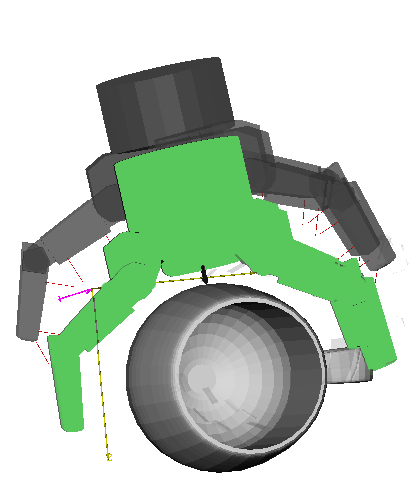
\includegraphics[height = 80mm]{initial_pose.png}
\caption{ \emph{Illustration of the initial pose and posture}. The hand begins in the green position and is withdrawn along its approach direction and all of the fingers opened at the same constant velocity until each of the fingertips are outside of the knuckles of the hand in its pre-grasp configuration. The hand is then opened an additional ten percent of the remaining joint range. This starting position is shown in black.}
\label{fig:initial_pose}
\end{figure}

\subsection{Model of Pose Uncertainty}
\label{sec:UncertaintyModel}
Because it is computationally intractable to densely sample the full six dimensional space of poses near the planned
pregrasp pose, we consider a three dimensional error model representing an object on a support surface. We assume that
each object is restricted to a set of stable poses on the surface.
\begin{figure}[b!]
\begin{centering}
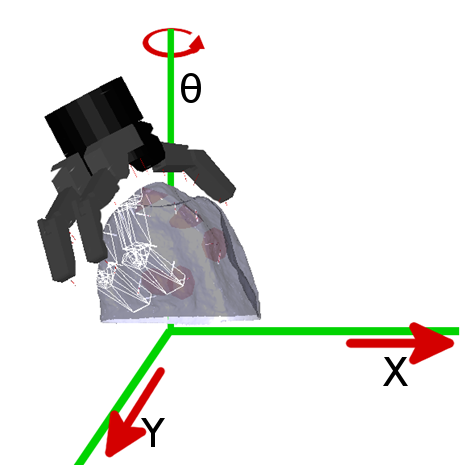
\includegraphics[height = 100mm]{ErrorModelIllustration.png}
\caption{Illustration of the tabletop error model used in this paper.  The object is can be translated $[-10,10]$ mm in both X and Y and rotated $[-20,20]^\circ$ around $\theta$.  The red cones mark the planned contact points.  The white wire frame indicates the planned end configuration of the fingers.}
\label{fig:errormodelillustration}
\end{centering}
\end{figure}
This error model is parametrized by $[x,y, \theta]$ as illustrated by Fig. \ref{fig:errormodelillustration}.  We use the centroid of the planned contact locations as the  origin of the object because parameterizing the rotation around the center of mass of the object will have a disproportionate effect on grasps planned further from the center of mass.  We chose bounds for the error model that were motivated by our anecdotal experience in aligning a known object to a point cloud using common methodologies. A reasonable range to explore using this parametrization should allow each parameter to move the relative position of the planned grasp's contact point by at least 10 mm.  If we make the rough approximation that the projection of the contact points perpendicular to the axis of rotation lie on a circle with a 5 cm radius, a reasonable range for these parameters is $\theta \in [-20^{\circ},20^{\circ}]$  and $x,y \in [-10 $mm$ ,10 $mm$]$.   Exploring this parameter space uniformly in increments of 1[mm,$^\circ$] in simulation requires 18,081 simulations per grasp. Using the GraspIt! grasping simulator\cite{Miller2004} on a Xeon 2.67GHZ processor we can perform this many kinematic simulations of the grasping pipeline in under two hours  for the worst case.  The time required for each simulation is object and grasp dependent. With cluster computing this approach can be used to analyze large numbers of grasps from a database off-line.\par

\subsection{Simulation Results}
These simulations resulted in a large dataset of grasps, perturbations from planned positions, and associated quality functions. From this data, we sought to answer two questions. First, how well do the quality measures of the planned grasp predict expected grasp qualities after perturbation. Second, how do grasp qualities affect the probability of attaining a \emph{force closed} grasp in the presence of pose uncertainty.  
\subsubsection{Expected Grasp Quality}
The grasps we analyzed were produced by the optimization procedure described in section \ref{sec:implications_for_robustness}. As we argued previously, it is reasonable to expect that the grasps produced by that planner should be locally near optimal with respect to the hand position. The resulting planned grasps are thus locally optimal with respect to the pose of the hand. To quantify how much the imposed pose perturbation affects a particular grasp, we can look at the expected value and standard deviation of its $\epsilon_{GWS}$ and $V_{GWS}$. However, to understand these effects on average across many grasps and objects, we normalize the expected value and standard deviation of these qualities by the quality values of the planned grasp with no error. We call the simulated quality measures of the planned grasp with no error the 'planned' quality values. Because the planned quality values are locally optimal, the expected value of the quality normalized to the planned value should have a maximum value of 1 for very robust grasps and a minimum value of 0 for extremely fragile grasps. We then consider the average of these quantities across all of the analyzed grasps. \par

\subsubsection{Probability of Achieving Force Closure}
\label{sec:successfraction}
Another important measure that contributes to grasp success is how likely the perturbed grasp is to fail to be \emph{force-closed}(\emph{fc}), which is defined as having an $\epsilon_{GWS}=0$.  These grasps are expected to be fundamentally unstable, and so a grasp with a higher average quality but a larger variance, leading to more non-\emph{fc} positions may succeed less often than a grasp with a lower average quality that has lower variance. To measure this effect directly, we counted the number of \emph{fc} grasps of the perturbed samples and divided that by the total number of samples, giving us a measure we have called $P(fc)$, as it represents the probability of achieving an \emph{fc} grasp given that our sampled perturbations are uniformly likely. 

Calculations involving convex hulls, such as the $\epsilon_{GWS}$ are known to be sensitive to numerical inaccuracies, and the cluster we used to generate this dataset was heterogeneous in both hardware and software environments. This initially lead to grasps that appeared \emph{fc}  with a small $\epsilon_{GWS}$ values to appear non-\emph{fc} when evaluated on a different machine in the cluster. To achieve consistent results, we had to choise an arbitrary small positive $\delta$ that is larger than the cross-machine variability that we observed, and redefine \emph{fc} to require that  $\epsilon_{GWS} > \delta$. In this work, we arbitrarily chose $\delta > 0.001$, as this was several orders of magnitude above the largest discrepancy we ever observed between two machines analyzing the same grasp, and several orders of magnitude lower than the quality of the average unperturbed grasp that we evaluated. 

We calculated these statistics across all of our grasps. These results are summarized in Table \ref{tab:expresultbrief}. We see that the expected $\epsilon_{GWS}$ and $V_{GWS}$ are 50\% and 67\% of their planned values, respectively.  This shows that pose uncertainty has a large effect on the expected value of these measures.  Additionally, we see that there is relatively high variance of these measures across all of the sampled perturbations for a single grasp. The average standard deviation of the measures across the perturbed samples of a single grasp is 29\% of the $\epsilon_{GWS}$ and 35\% of the $V_{GWS}$. 

The observation that the within grasp variability is high is what led us to consider whether the number of non-$fc$ perturbed samples varied significantly across grasps with similar $\epsilon_{GWS}$ qualities. We found that the average $P(fc)$ is around 80\%. This implies that even the best five grasps for the object should be expected to fail 20\% of the time, if we only filter grasps by their $\epsilon_{GWS}$  quality.

\begin{table}
\begin{tabular}{ |c |c |}
\hline
Measure across sampled perturbations&Average across 'Tool' grasp dataset\\ \hline
normalized expected ${\epsilon}_{GWS}$&0.5091 \\ \hline
normalized std(${\epsilon}_{GWS})$&0.2915 \\ \hline
normalized expected $V_{GWS}$&0.679 \\ \hline
normalized std($V_{GWS})$&0.3588 \\ \hline
$P(fc)$&0.7957\\ \hline
\end{tabular}
\caption{Summary of Simulation Results: These results quantify how robust each quality measure is to pose uncertainty. For each grasp, the expected value and standard deviation of the respective quality measures are calculated across the poses sampled.  These measures are normalized by dividing them by the planned quality of the unperturbed grasp to allow comparison of the effects of uncertainty across grasps. $P(fc)$ denotes the measured probability of achieving an \emph{fc} grasp, which we have calculated as $P(\epsilon_{GWS} >.001) $ }.
\label{tab:expresultbrief}
\end{table}

\subsection{Choosing Optimal Grasps: $\epsilon_{GWS}$ vs $P(fc)$}
In the case of choosing a single grasp out of a set of many, we are faced with the problem of ranking grasps. The fundamental question we seek to answer with this research can be rephrased simply as whether performing that ranking relying solely on the $\epsilon_{GWS}$ is sufficient to chose the grasp most likely to achieve stable \emph{force closure} in the presence of location uncertainty. 


\begin{figure}
\centering
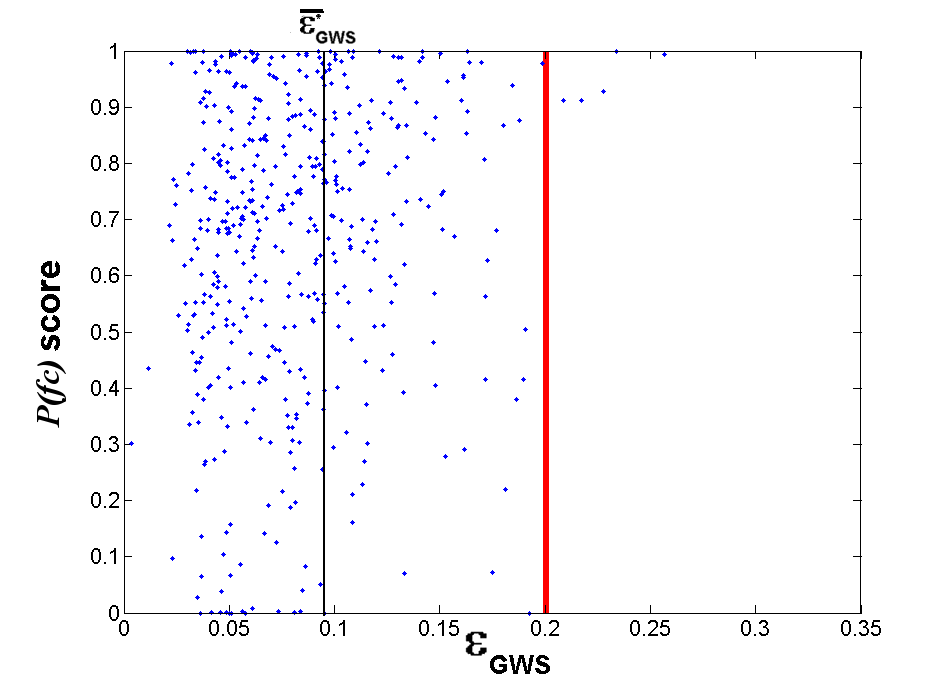
\includegraphics[height = 100mm]{tooleps_annotated.png}
\caption{$\epsilon_{GWS}$ plotted against $P(fc)$, which is equivalent to the probability of attaining an \emph{fc} grasp under our error model from a planned starting grasp configuration.  480 grasps over 96 objects are presented in this figure. This figure demonstrates that the $\epsilon_{GWS}$ is generally a poor predictor of pose error robustness as measured by the $P(fc)$.  The mean $\epsilon_{GWS}$, denoted by the black line, is 0.095.  There appears to be a cutoff, denoted by a red vertical line on the graph,  around $\epsilon_{GWS} > 0.2$, after which all available grasps are have a high $P(fc)$, but note how few grasps there are in the database with quality values that high. Only five objects have a grasp with a quality that high, which implies that for most objects, $\epsilon_{GWS}$ cannot be used to predict $P(fc)$. }
\label{fig:sp-vs-epsilon}
\end{figure}


 In Fig. \ref{fig:sp-vs-epsilon}, we have plotted the planned $\epsilon_{GWS}$ against the estimate of the probability of achieving force closure, for each grasp.   $\overline{\epsilon^*}_{GWS}$ indicates the average $\epsilon_{GWS}$ for the best grasp available for each object, which is 0.095. For most objects, the best grasp by $\epsilon_{GWS}$ lies in the range where $\epsilon_{GWS}\in(0, 0.2)$, bordered by the red line on the right of the figure.  This figure shows that there is no correlation between $\epsilon_{GWS}$ and $P(fc)$ in that range. 
 
 This implies that the $\epsilon_{GWS}$ cannot be used to chose grasps that are expected to be robust. On average the best grasp by $P(fc)$ for each object has a $P(fc)$ that is 0.21 greater than the $P(fc)$ of the highest $\epsilon_{GWS}$ grasp. Under the error model described, choosing the highest $P(fc)$ grasp will result in an \emph{fc} grasp 21\% percent more often than choosing the best grasp by $\epsilon_{GWS}$. This analysis yields approximately the same results for the $V_{GWS}$ in comparison to the $P(fc)$.\par

\section{Physical Experiments}
These simulation results show that using $P(fc)$ as a quality metric for ranking grasps from a database may select grasps that are more reliable in the face of object pose estimation error. To test whether these simulation results can be verified against physical experiments, we attempted to grasp ten objects for which we had high quality mesh models readily available courtesy of the the DARPA ARM-S project and the Willow Garage object database [23]. We added these models to our database, and calculated the $P(fc)$ for the top five grasps by $\epsilon_{GWS}$ value.

 To test these grasps on a real robotic grasping system we used a Barrett 280 model hand attached to a Staubli TX60L 6 degree of freedom arm to implement the grasping pipeline described in \ref{sec:GraspingPipeline}. To emulate the friction coefficient used in our simulations, we wrapped the contacting surfaces of the hand in rubberized shelf liner. One object attempted was a blue detergent bottle made of very smooth plastic. We added a rubberized tape to the contact locations on this object to increase its friction coefficient. For each object, we selected the best grasp ranked by $\epsilon_{GWS}$ and the best grasp ranked by $P(fc)$. The objects were calibrated to the robot using a printed template of the bottom outline of the objects. We align the edge of each template to a known coordinate system in our robot’s workspace. We selected a perturbed position by sampling our error model and then applying the grasp pipeline as though the object’s origin was at the perturbed location. 

We tested up to ten randomly selected perturbed positions for each grasp. The same perturbations were applied to both of the tested grasps for each object. We moved the arm and hand at very slow speeds to simulate quasi-static conditions. In the first two stages of the pipeline, we moved the arm at 1\% of its maximum speed, and the fingers of the Barrett hand at 10\% of their maximum speed. In the final closing step, initial contact had been achieved or joint limits had been reached for each finger. We then raised the finger speed to 50\% to drive the underactuated fingers to their final positions. After the fingers stopped moving, we lifted the object 3 cm perpendicular to the table’s surface. If any part of the object was still touching the table when the arm came to a stop, we graded the trial as a failure, otherwise we graded the trial as a success. 

We find that the grasps ranked best by the $P(fc)$ are successful more often. The results of this experiment along with the grasps and objects analyzed are in Fig. \ref{fig:fgrasps_large} and Fig. \ref{fig:fgrasps_small}. Overall, for these ten objects the $P(fc)$ ranking selected successful grasps on 85 out of 93 trials (91\%), whereas the grasps selected by the $\epsilon_{GWS}$ ranking succeeded on 63 of 93
trials (67\%).
For some objects, nearly all of the grasp attempts were successful irrespective of the $P(fc)$ score. We separated the objects in our experiment into two groups. One group is composed of of larger, more complex objects shown in Fig. \ref{fig:fgrasps_large} and the other group is composed of light, roughly cylindrical objects shown in shown in Fig. \ref{fig:fgrasps_small}. We see that all of the objects in the roughly cylindrical category were grasped very robustly irrespective of $P(fc)$ score. For these objects, the Eigengrasp planner finds grasps that more or less encompass the object. In contrast, for the five objects that could not be enveloped by the hand, we see that the $P(fc)$ ranked grasp is successful in 35 out of 43 trials (81\%), as compared to 16 out of 43 trials (37\%) using the $\epsilon_{GWS}$ grasp. These results show that the $P(fc)$ ranking chooses more successful grasps; especially on the larger, more complex objects where the success rate is doubled.

\begin{figure}
\centering
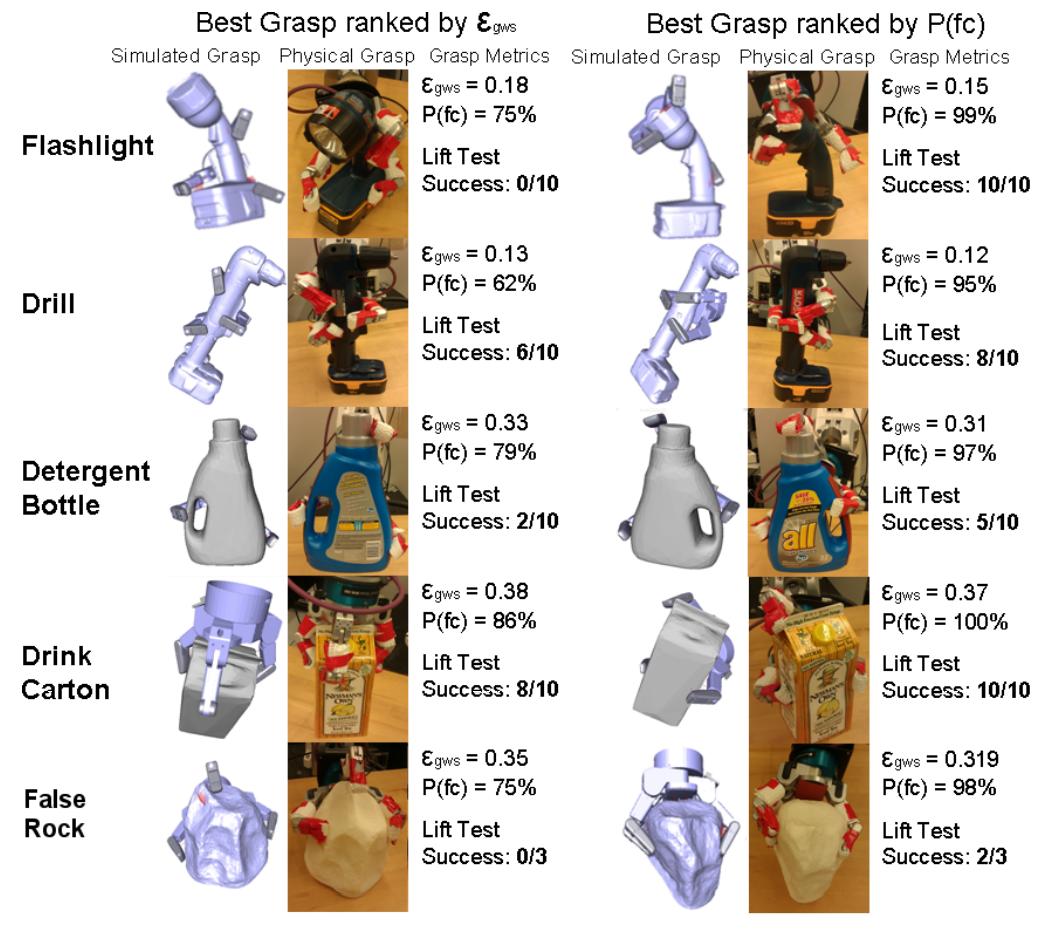
\includegraphics[width=\linewidth]{pfc_physical_grasps_large.png}
\caption{\emph{Results A:} The results of physical experiments on five large, complex objects. In the left column are the best grasps for each object ranked by $\epsilon_{GWS}$. An example of the simulated and physically realized grasp is illustrated for each grasp attempted. Additionally, the figure gives the $P(fc)$ and  $\epsilon_{GWS}$ for each grasp attempted, as well as the fraction of attempts which succeeded in lifting the object by 3 cm in physical experiments. The higher $P(fc)$ grasp is successful on many more trials than the higher  $\epsilon_{GWS}$ grasp for these objects.}
\label{fig:fgrasps_large}
\end{figure}

\begin{figure}
\centering
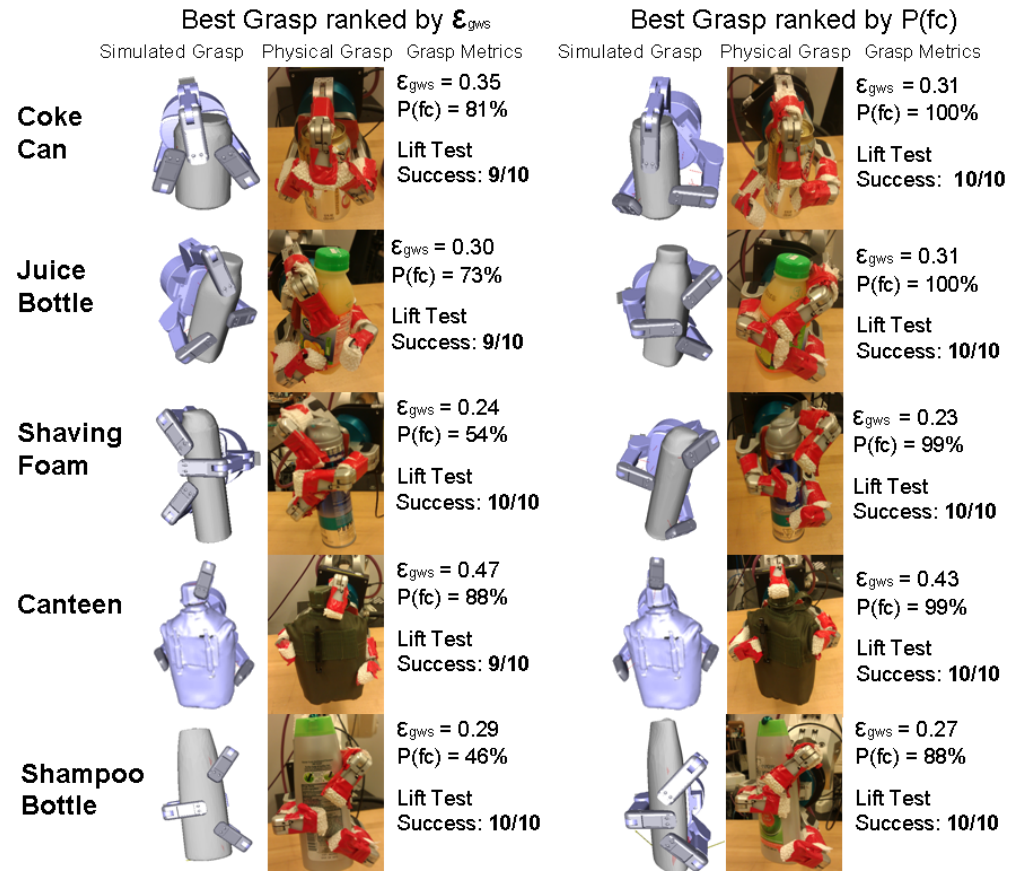
\includegraphics[width=\linewidth]{pfc_physical_grasps_small.png}
\caption{\emph{Results B:} The results of physical experiments on five smaller, simpler objects. In the left column are the best grasps for each object ranked by $\epsilon_{GWS}$. In the right column are the best grasps by $P(fc)$. An example of the simulated and physically realized grasp is illustrated for each grasp attempted. Additionally, the figure gives the $P(fc)$ and $\epsilon_{GWS}$ for each grasp attempted, as well as the fraction of attempts which succeeded in lifting the object by 3 cm in physical experiments.}
\label{fig:fgrasps_small}
\end{figure}
 

\section{Discussion}
\label{discussion}
In this work, we have shown that the planned $\epsilon_{GWS}$ of a planned grasp is not predictive of the probability of achieving a force closed grasp in the presence of uncertainty, neither in simulation nor physical experiments. To analyze this in simulation we generated the measure $P(fc)$ as an approximation of this probability. We then showed that the $P(fc)$ can itself be used to rank grasps from a preplanned grasp database and that this reranking predicts grasping success in physical
experiments better than the $\epsilon_{GWS}$ . 

The analysis presented here is less effective at discriminating fragile grasps on smaller objects than it is on larger objects. For small objects, the object is fully encompassed by the hand, and the highest $\epsilon_{GWS}$ grasp is always an enveloping power grasp, and is always spherical, as described in \cite{Cutkoskytaxonomy}. As seen in Fig. \ref{fig:fgrasps_small}, in such grasps the palm is behind the object, one finger pressing downwards, with fingers roughly evenly spaced apart. For a hand capable of achieving this configuration, it is always a high $\epsilon_{GWS}$ grasp, because the normals of the contact points are evenly spaced around the center of the grasp, which maximizes their ability to directly oppose perturbation forces. It is also a configuration that is relatively invariant to perturbations that do not move the object outside of the working envelope of the hand. 

Under more constrained conditions, such grasps are not always attainable. The object may not be in the center of the workspace, there may be objects in the way, or the desired purpose to which the object will be put requires a different grasp. These cases are better represented by the results on the large objects, which couldn't be fully encompassed by the hand. Under these conditions, the higher $\epsilon_{GWS}$ grasp often fails, and we see better results ranking by $P(fc)$.

\subsection{Online Extensions}

\begin{table}
\centering
\begin{tabular}{ |c |c | c | c | }
\hline
Sampling Step Size (X, Y, $\theta$) & Mean Difference & Standard Deviation & Max Difference \\ 
 (mm, mm, $^{\circ}$ &  & &\\ \hline
2-2-4 & 0.0128 & 0.0122 & 0.0667 \\ \hline
2-2-4(random) & 0.0097 & 0.0086 & 0.0493  \\ \hline
10-10-10 & 0.0653 & 0.0551 & 0.3205  \\ \hline
10-10-20 & 0.0840 & 0.0713 &0.4782 \\ \hline
\end{tabular}
\caption{This table quantifies the effect of sampling parameters on the estimate of quality measure
The first column describes the sampling density along each dimension of the error model. The other columns describe the average change in the subsampled $P(fc)$ as compared to the densest sampling rate. These results demonstrate that lower sampling rates may feasibly be used to approximate the $P(fc)$ at the densest sampling rate without unacceptable loss of accuracy.}
\label{tab:expresultbrief2}
\end{table}


Although the full sampling rate is too computationally expensive, in Table \ref{tab:expresultbrief2} we examine the possibility of approximating $P(fc)$ at lower sampling rates. By using a sampling step size of (10mm, 10mm, 10$^\circ$), we see an average difference of 6\% with respect to the denser sampling. In none of our samples did this change the order of our rankings. At this sampling rate, we can generate an estimate in under a second, which make it suitable as a filter for an online grasp planning system. At lower sampling rates, the rankings do become reordered, which may lead us to select less robust grasps. In our shared control online planner, we use the lower resolution $P(fc)$ to weight the grasp quality measure that controls the order in which grasps are tested for reachability, and the order in which they are presented to the user. Without this filter, many grasps that are presented to the user are fragile to object pose estimation errors.   

In Chapters 4-6, we have will demonstrate an online planner that uses a human-in-the-loop with an extremely limited interface to act as a second filter selecting the appropriate grasp. When the grasps that are presented include many fragile grasps, more of the responsibility is placed on the user, which requires both more insight and more interaction. Since the bitrate and accuracy of the interfaces we will use is limited, reducing the number of inappropriate grasps can help reduce training time, and improve the speed and accuracy of the system.  By filtering out non-robust grasps, we are able to present the user with a more suitable set of grasps that they can manage even with a limited interface. 
